\header{
    \section{Catin, catin, aimable catin} \label{catin-catin-aimable-catin}
    %
    
    \insertComment{Catin est le diminutif ancien de Catherine}{}
}

\enluminure{4}{\href{}{C}}{atin}, Catin, aimable Catin
\\Que fais-tu dans ce jardin ?
\\- J'rammass' des fleurs
\\De toutes les couleurs
\\Pour en faire un beau présent
\\Pour en faire un beau présent
\\A mon fidèle amant
\\\\Catin, Catin, aimable Catin
\\M'en donnerais-tu pas un ?
\\- Entrez dans mon jardin
\\Vous en choisirez
\\De ces beaux lauriers
\\Ceux qui font penser à vos yeux
\\Ce que vous aimez le mieux.
\\\\Ce ne sont pas tes beaux lauriers
\\La belle qui m'ont charmé.
\\C'est ton tendre coeur
\\Et tes forts beaux yeux
\\Je suis amoureux.
\\Veux-tu venir dans la cour
\\Le restant de tes jours
\\\\Je suis fille sans rien
\\Je n'ai aucun bien
\\Ni aucun entretien
\\Vous ne voudriez pas épouser
\\La fille d'un jardinier
\breakpage
\\\\Pourquoi ne t'épouserais-je pas
\\La belle si tu m'aimais
\\J'ai un beau diamant
\\Qui vaut mille Francs
\\Je t'en fais présent
\\Et tu seras la femme d'honneur 
\\La dame d'un grand seigneur
\\\\Je suis fille sans rien
\\Je n'ai aucun bien
\\Ni aucun entretien
\\Vous ne voudriez pas épouser
\\La fille d'un jardinier
\\\\Adieu jardin adieu cour
\\Adieu pour toujours
\bisquintuple{Je vois un beau jardin}
{De fleurs entouré,}
{Je te quitte enfin}
{Je m'en vais suivre mon amant}
{Qui m'aime tendrement}

\bigskip
\begin{figure}[h!]
\centering
   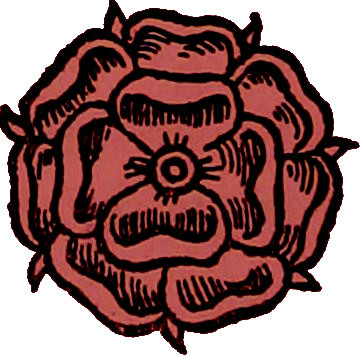
\includegraphics[width=0.5\textwidth]{images/brev47.png}
 \end{figure}
 

\breakpage